\subsection{Find patient gender from XRay(s)}
\label{sec:warmup3}

    In this preliminary practice activity, we were given chest X-ray images of patients using which we have to either train or fine-tune a model to determine the gender of patients.

\subsubsection{Dataset}
\label{sec:orienattion-dataset}
    We were given three datasets for classifying gender of the patients; grayscale, RGB, and index. Out of these, I have used grayscale images for the experiment. The provided dataset have 154 training samples of patient X-Rays and an additional 93 samples for testing the trained model.  The images in this dataset were color image with shape $256 \times 256$. Each training samples have either label "male", or "female". Due to the absence of a dedicated validation set in this dataset too, I have randomly partitioned the training samples into training and validation sets in 9:1 ratio.

\subsubsection{Training}

    In this task, we are dealing with two labels; male and female. Therefore, I have constructed a model with resnet18 as feature extractor, and the model graph is described in \cref{fig:gender_model}. A sigmoid layer is employed as the last activation function to get the output in range of $0-1$. The model is trained using the binary cross-entropy loss function with adam optimizer with a learning rate of $3.0 \times 10^{-4}$. The model was trained for a total of $20$ epochs. \Cref{fig:gender-learning-curve} illustrates the learning curve of the training and validation sets.

    \begin{figure}[htbp]
        \centering
        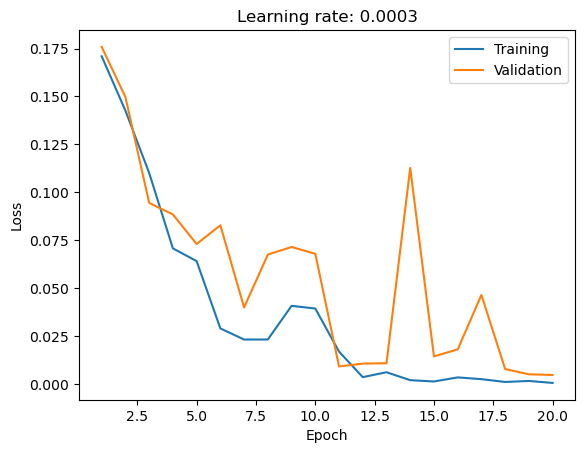
\includegraphics[width=\linewidth]{../plots/gender/learning.png}
        \caption{Learning curve of model trained on chest xray gender dataset.}
        \label{fig:gender-learning-curve}
    \end{figure}

\subsubsection{Results}

    \begin{figure*}[!htbp]
        \centering
        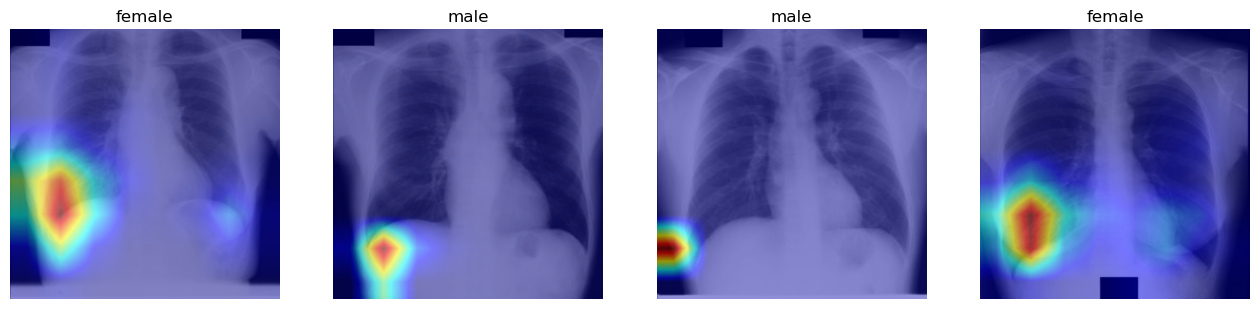
\includegraphics[width=\linewidth]{../plots/gender/result.png}
        \caption{Gender predections on few test samples with GradCAM visualization.}
        \label{fig:gender-results}
    \end{figure*} 

    After fine-tuning the model, it was evaluated on the provided test samples, and \cref{tab:classification-model-results} reports the achieved accuracy and AUC. \Cref{fig:gender-results} showcases some of the test samples along with their model predictions and target classes. The figure also includes GradCAM visualizations generated using the last layer of the ResNet18 backbone. The GradCAM visualization is helpful for understanding why the model classified certain images into specific classes.
